\documentclass[twocolumn]{revtex4}

\usepackage{graphicx}
\usepackage{amsmath}

\begin{document}

\title{Classical simulation of liquid argon}
\author{David Stygstra}

\maketitle

\section{Introduction}

Liquid argon can be classically simulated by placing argon atoms with velocities in a Maxwell-Boltzmann distribution (section~\ref{sec:vel-dist}) in a Lennard-Jones potential (section~\ref{sec:lj}), then solving Newton equations with respect to time (section~\ref{sec:verlet}).

A number of properties can be observed in this system, including:

\begin{itemize}
\item Temperature (section~\ref{sec:temp})
\item Total energy (sections~\ref{sec:ke} and ~\ref{sec:lj})
\item Position (section~\ref{sec:msd})
\item Velocity (section~\ref{sec:vel-dist})
\end{itemize}

\section{Computational method}

Argon atoms are placed in a crystal structure at a given temperature, then evolved in time while logging a number of properties of the system.

\subsection{Initialization}

\subsubsection{Crystal structure}

The atoms are placed in a face-centered cubic (FCC) configuration, where each ``unit cell'' consists of 4 atoms positioned as illustrated in figure~\ref{fig:fcc}. A collection of argon atoms in an $L \times L \times L$ box with $d$ FCC unit cells in each direction thus has a number density of $n = 4d^3/L^3$.

\begin{figure}[htb]
\begin{center}
\leavevmode
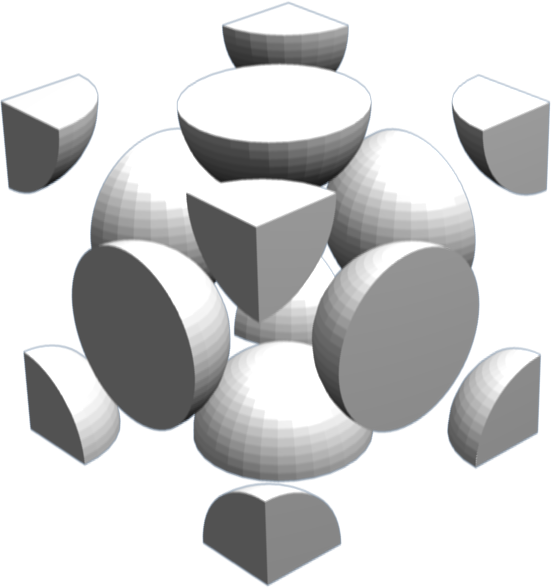
\includegraphics[width=0.45\textwidth]{fcc.png}
\end{center}
\caption{Face-centered cubic (FCC) lattice unit cell.}
\label{fig:fcc}
\end{figure}

\subsubsection{Velocity distribution}
\label{sec:vel-dist}

The velocity of each argon atom is set according to a Maxwell-Boltzmann distribution---i.e., a Gaussian distribution for each axis of the velocity. I used the Box-Muller algorithm to generate Gaussian-distributed numbers:

\begin{align}
z_1 &= \sqrt{-2 \ln u_1} \cos{2 \pi u_2}\\
z_2 &= \sqrt{-2 \ln u_1} \sin{2 \pi u_2},
\end{align}

where $u_1, u_2$ are uniformly distributed random numbers on $(0,1]$ and $z_1, z_2$ are Gaussian distributed random numbers. This causes the argon atoms to have speeds distributed with a Maxwell-Boltzmann distribution as shown in figure~\ref{fig:vel-dist}.

\begin{figure}[htb]
\begin{center}
\leavevmode
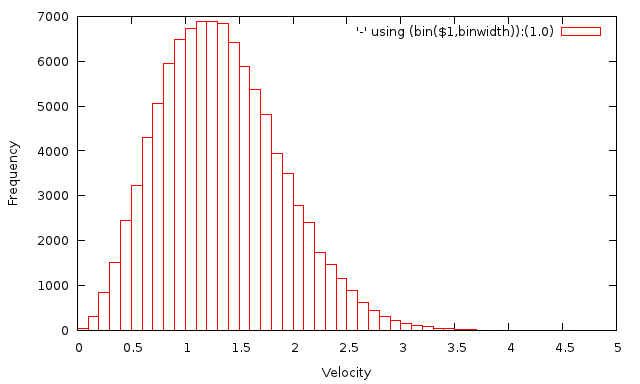
\includegraphics[width=0.45\textwidth]{vel-dist.png}
\end{center}
\caption{Maxwell-Boltzmann speed distribution of $10^4$ argon atoms at a temperature of 0.7 TU = 84 K.}
\label{fig:vel-dist}
\end{figure}

The velocities of the atoms are then scaled by a factor of $\sqrt{T_{\text{target}}/T}$ to bring the system to its target temperature.

\subsection{Simulation}

\subsubsection{Lennard-Jones potential}
\label{sec:lj}

The argon atoms are placed in a Lennard-Jones potential so that the potential of two atoms separated by a distance $r$ is

\begin{align}
V = 4\varepsilon \left( \left(\frac{\sigma}{r}\right)^{12} - \left(\frac{\sigma}{r}\right)^6 \right),
\end{align}

where $\sigma \approx 3.405\cdot10^{-10}$ m, $\varepsilon \approx 1.654\cdot10^{-21}$ J, and the mass $m \approx 6.69\cdot10^{-26}$ kg for argon. In the simulation, the units are normalized so that $\sigma = \varepsilon = m = k_B = 1$, so the potential is:

\begin{align}
V = 4 \left( \left(\frac{1}{r}\right)^{12} - \left(\frac{1}{r}\right)^6 \right).
\end{align}

The force on an atom is determined by the distances to all other atoms:

\begin{align}
\mathbf{f}_{i} = -24 \sum_{j\ne i} \left( \frac{2}{r_{ij}^{14}} - \frac{1}{r_{ij}^8} \right),
\end{align}

where $\mathbf{f}_i$ is the force on particle $i$ and $r_{ij}$ denotes the distance from particle $i$ to particle $j$.

\subsubsection{Verlet algorithm}
\label{sec:verlet}

The simulation steps forward using the Verlet algorithm:

\begin{align}
X_{t+\delta t} &= X_t + V_t \delta t + F_t \frac{\delta t^2}{2}\\
F_{t+\delta t} &= \text{Lennard-Jones}(X_{t+\delta t})\\
V_{t+\delta t} &= V_t + (F_{t+\delta t} + F_t) \frac{\delta t}{2},
\end{align}

where $X$, $F$, and $V$ are matrices representing the positions, forces, and velocities of each argon atom. The subscript on each of these matrices denotes the simulation time the matrix represents the state of---for example, $X_{t+\delta t}$ represents the positions of the particles at $\delta t$ time units after the time $t$.

\subsubsection{Periodic boundaries}

In order to simulate a larger system, the simulation uses periodic boundary conditions; i.e., the atoms lie in a three-dimensional torus. However, this can cause the particles to attain a ``drift'', or non-zero center of mass velocity, due to numerical errors. To counteract this, the center of mass velocity of the system is zeroed before each timestep.

\subsection{Observable values}

\subsubsection{Kinetic energy}
\label{sec:ke}

To find the kinetic energy, the squared velocities of the atoms are summed up and divided by 2. Because $m=1$ (by definition), that term is removed.

\begin{align}
KE = \frac{1}{2} \sum_i m_i |\mathbf{v}_i|^2 = \frac{1}{2} \sum_i |\mathbf{v}_i|^2
\end{align}

\subsubsection{Temperature}
\label{sec:temp}

The temperature is calculated by the kinetic energy with

\begin{align}
\frac{3}{2} (N-1) k_B T &= \frac{1}{2} \sum_i |\mathbf{v}_i|^2 = KE\\
\implies & T = \frac{2}{3 k_B (N-1)} KE.
\end{align}

\subsubsection{Mean square displacement}
\label{sec:msd}

In order to track the mean square distance of each atom from its original position, the simulation uses an extra variable $\mathbf{disp}$ that keeps track of a atom's displacement regardless of periodic boundary conditions. The mean square displacement is then defined as

\begin{align}
MSD = \frac{1}{N} \sum_i |\mathbf{disp}_i|^2 = \frac{1}{N} \sum_i |\mathbf{x}_t - \mathbf{x}_0|^2.
\end{align}

\section{Results}

\subsection{Test of two atoms in a Lennard-Jones potential}

In order to make sure the Lennard-Jones potential and Verlet algorithm function correctly, I implemented a test case with two argon atoms separated by a distance of 2 length units ($7\cdot10^{-10}$ m) in a Lennard-Jones potential. Figure~\ref{fig:lj-pos} shows the positions of the two argon atoms as a function of time---this shows the repulsive force of the potential at close ranges and the attractive force at farther ranges. Figure~\ref{fig:energy-cons} shows the total energy of the system as a function of time. Note that there is some instability when the atoms are close (strong forces lead to numerical errors), but the total energy returns to the correct value once the atoms are farther apart.

\begin{figure}[htb]
\begin{center}
\leavevmode
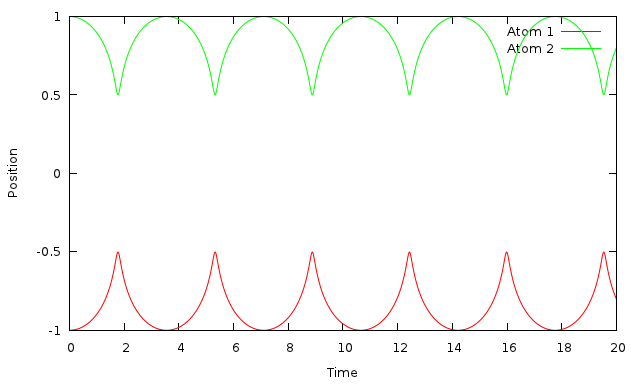
\includegraphics[width=0.45\textwidth]{lj-pos.png}
\end{center}
\caption{Position of two argon atoms in a Lennard-Jones potential.}
\label{fig:lj-pos}
\end{figure}

\begin{figure}[htb]
\begin{center}
\leavevmode
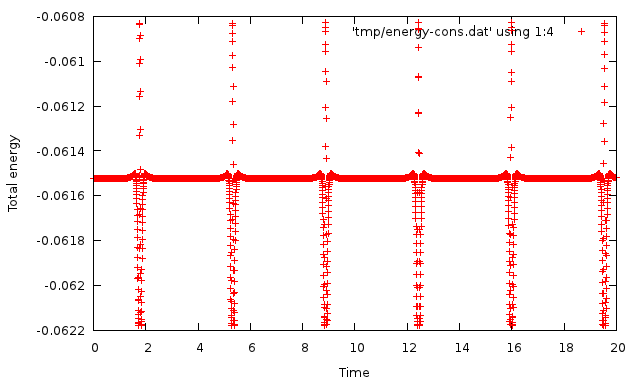
\includegraphics[width=0.45\textwidth]{energy-cons.png}
\end{center}
\caption{Total energy of a system with two argon atoms in a Lennard-Jones potential.}
\label{fig:energy-cons}
\end{figure}

\subsection{Energy-temperature relation}

To find an energy-temperature relation, I ran the simulation for a set of temperatures and found the total energy based on a number of Verlet iterations. The result fit well to a logarithmic curve of the form $E(T)=\ln(T/a)$ as shown in figure~\ref{fig:temp-response}.

\begin{figure}[htb]
\begin{center}
\leavevmode
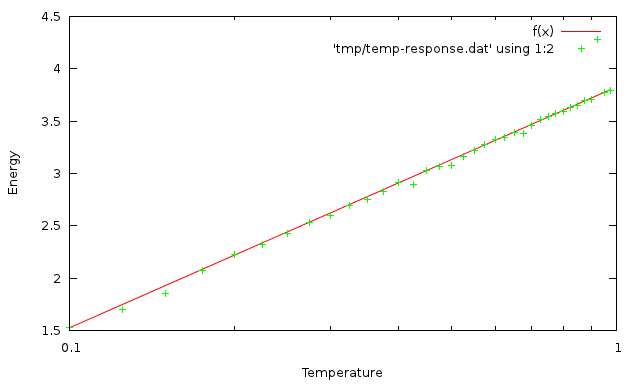
\includegraphics[width=0.45\textwidth]{temp-response.png}
\end{center}
\caption{Logarithmic relation of the temperature and total energy of a system. The logarithmic fit in the plot is defined by $E(T) = \ln(T/0.022)$. The temperature scale ranges from 12 K to 120 K and the energy scale ranges from $2.48\cdot10^{-21}$ J to $7.44\cdot10^{-21}$ J.}
\label{fig:temp-response}
\end{figure}

\subsection{Mean square displacement}

To generate figure~\ref{fig:avg-msd}, I ran the simulation for a set of temperatures and recorded the mean square displacement for each timestep. The result fit well to the surface $MSD(T,t)=aTt^2$, where $T$ is the temperature and $t$ is the time.

Each temperature ``cross-section'' fits a curve of the form $MSD(t)=bt^2$.

See section~\ref{sec:msd} for a description of how the mean square displacement is calculated.

\begin{figure}[htb]
\begin{center}
\leavevmode
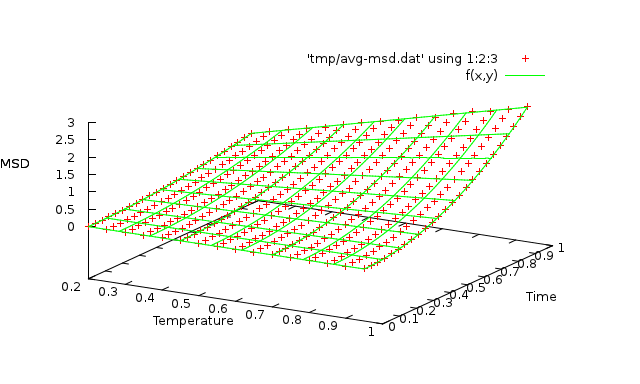
\includegraphics[width=0.45\textwidth]{avg-msd.png}
\end{center}
\caption{Mean square displacement as a function of temperature and time. The fit surface is described by $MSD(T,t)=2.85 T t^2$. Temperature scale: 24 - 120 K. Time scale: 0 - $2.17\cdot10^{-12}$ s. Length scale: 0 - $1.02\cdot10^{-9}$ m.}
\label{fig:avg-msd}
\end{figure}

\section{Note about units}

In section~\ref{sec:lj}, I defined $\sigma = \varepsilon = m = k_B = 1$. As a result of these definitions, the following unit system can be defined (where the right hand side contains the units used in the simulation):

\begin{itemize}
\item $3.405\cdot10^{-10}$ m = 1 LU (length unit)
\item $1.654\cdot10^{-21}$ J = 1 EU (energy unit)
\item $6.69\cdot10^{-26}$ kg = 1 MU (mass unit)
\item $1.199\cdot10^2$ K = 1 TU (temperature unit)
\item $2.17\cdot10^{-12}$ s = 1 tU (time unit)
\end{itemize}

So, for example, consider argon with a number density of $n=0.9$ LU$^{-3}$. The mass density $\rho = nm = 0.9\text{ MU/LU}^3 = 1.5\text{ g/cm}^3$.

Choosing units that keep the calculations away from extreme values (e.g. $10^{-25}$ or $10^{40}$) helps mitigate numerical errors due to the floating point representation of numbers.

\begin{thebibliography}{9}

\bibitem{duxbury2011-1}
	Phillip Duxbury,
	\emph{Molecular Dynamics Lecture 1}.
	\url{http://www.pa.msu.edu/~duxbury/courses/phy480/mdlecture1.pdf}
	(retrieved 2011-04-13)

\bibitem{duxbury2011-2}
	Phillip Duxbury,
	\emph{Molecular Dynamics Lecture 2}.
	\url{http://www.pa.msu.edu/~duxbury/courses/phy480/mdlecture2.pdf}
	(retrieved 2011-04-13)

\end{thebibliography}

\end{document}
